\chapter{Wing Box model} \label{chap:Model}

\section{Introduction} \label{sec:intro_Model}

% Introduction to the chapter

\section{Concept} \label{sec:concept_Model}

% Explanation of the concept
% -> Bending-twist coupling
% -> Shiftable shear centre location
% -> A web with variable-stiffness capability

% Figure: Fig. 1 Raither ?, Geometry and system of coordinates.
% Figure: Fig. 2 Raither ?, Schematic of the working principle.

% -> Buckling phenomena
% Figure: Schematic representation buckling phenomena

\section{Analytical model} \label{sec::analytical_Model}

%% Analytical apprach description
% An analytical model of the Wing Box will be build.
% Shear centre calculation
% The twist of the beam will be calculated
%
%Figure of analytical model
\begin{figure}[!htpb]
  \centering
  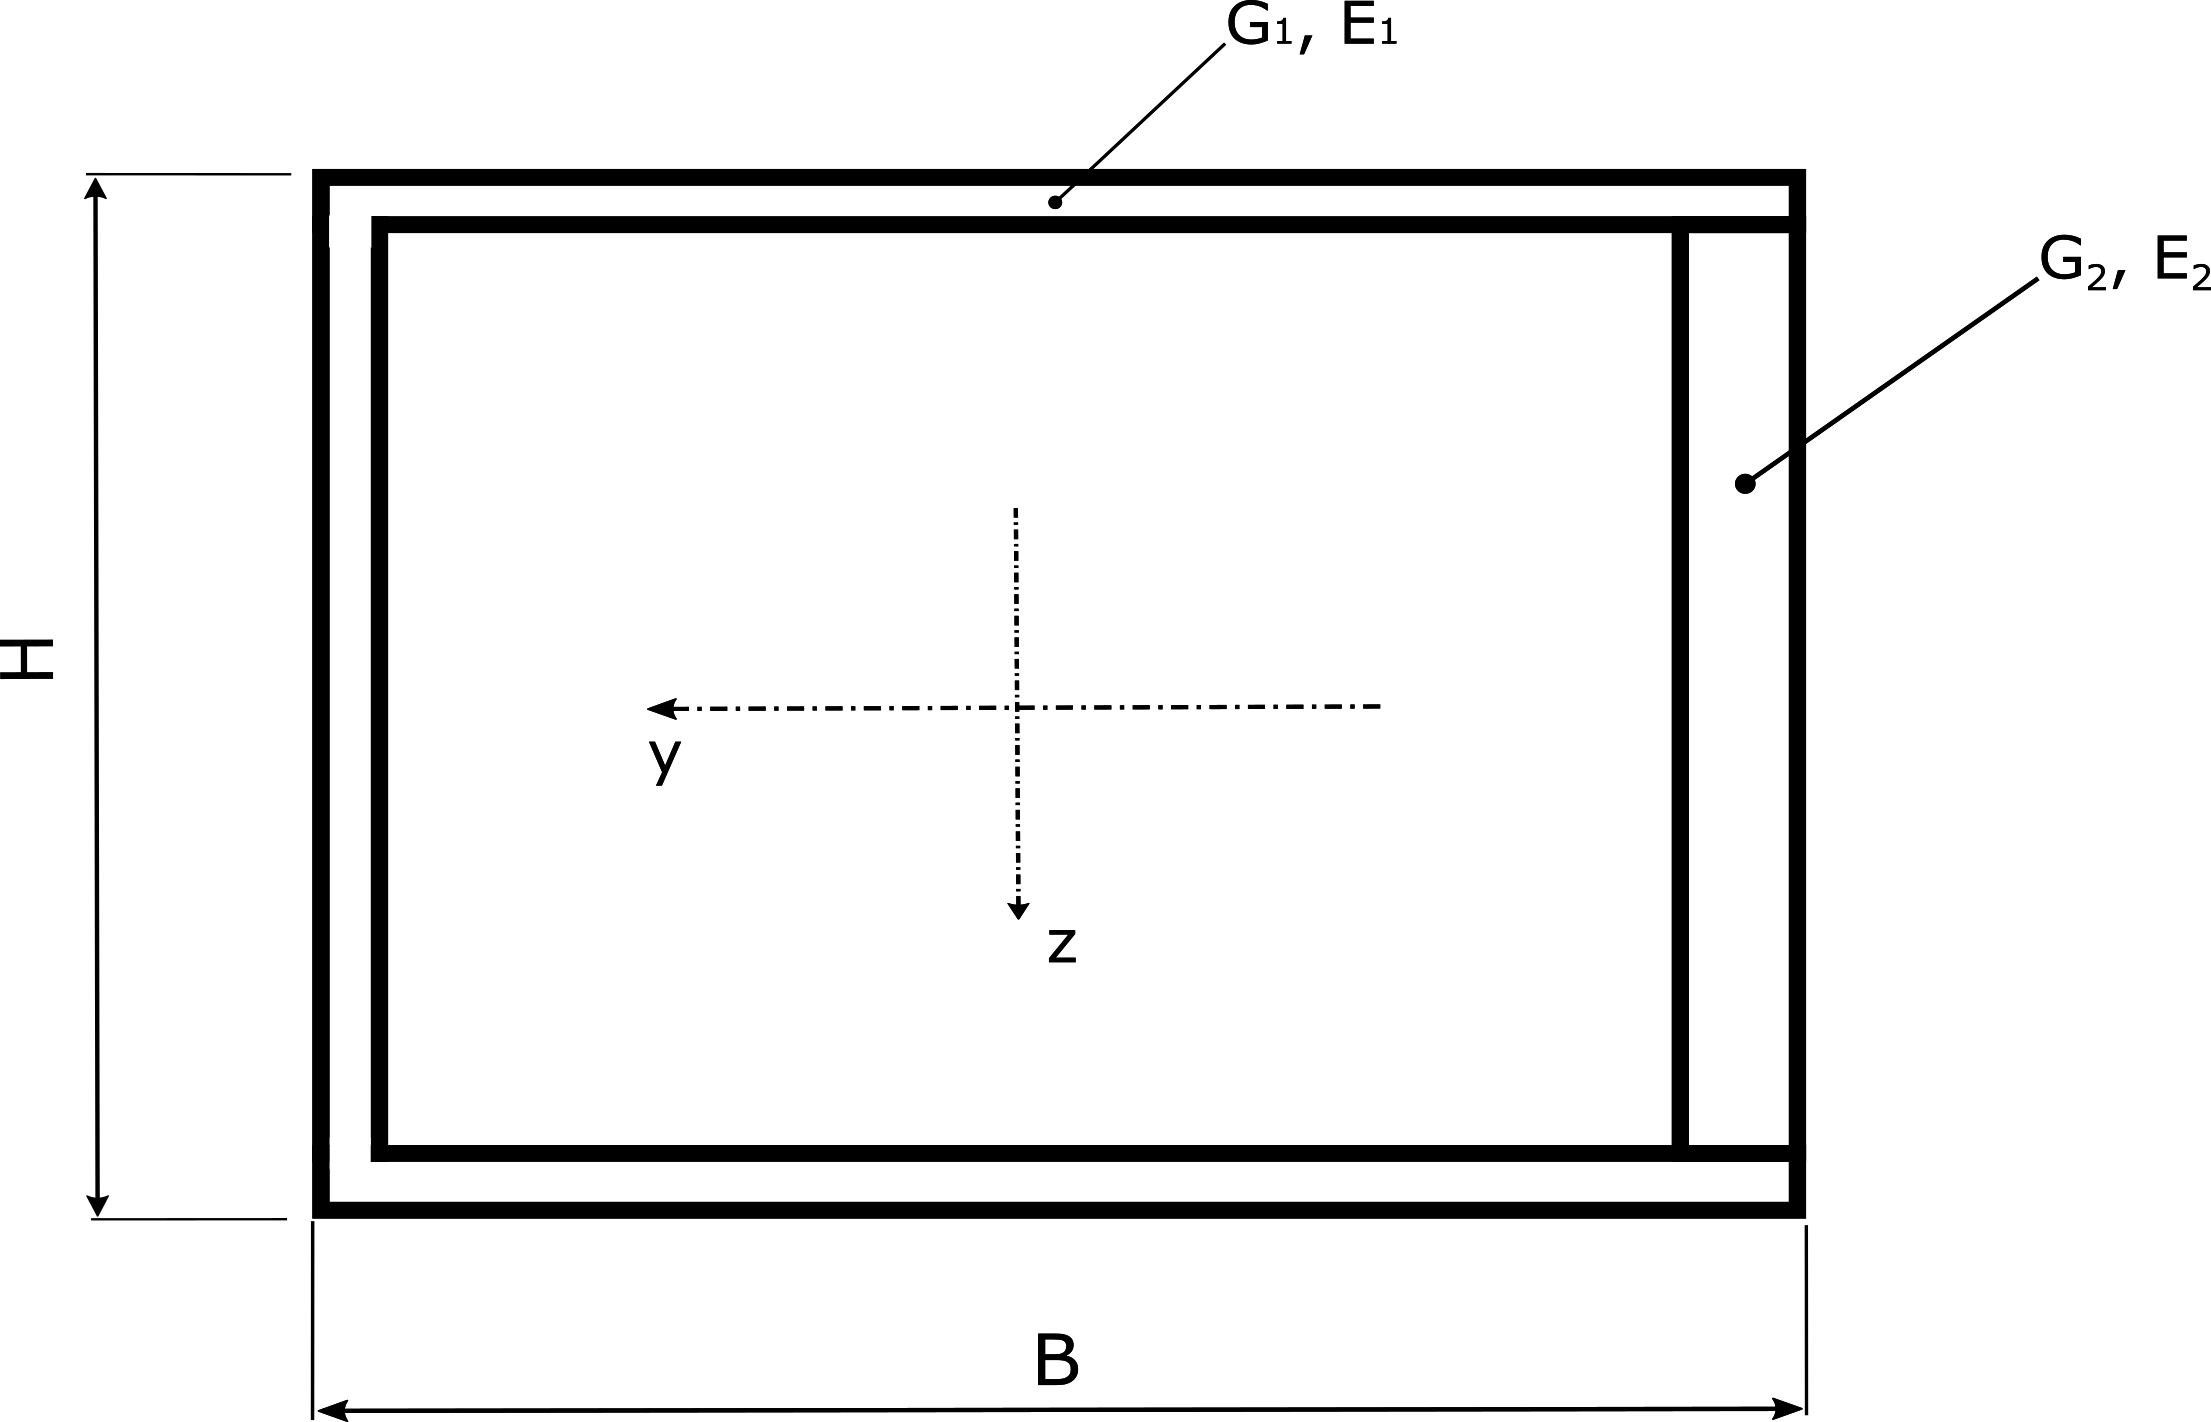
\includegraphics[width=0.8 \textwidth]{model/analyticalBox}
  \caption[Schematic view of the beam closed section]{Schematic view of the beam closed section. The dimensions are given by the width $B$ and the height $H$. For the upper, lower and left elements, the shear modulus and the elastic modulus are given by $G_1$ and $E_1$, respectively. For the right element, the same mechanical properties are given by $G_2$ and $E_2$.}\label{fig:analyticalBox}
\end{figure}

%Torsional stiffness

\begin{equation}\label{eq:torStiff}
  G I_t = \frac{4 A_0^2}{\oint \frac{\mathrm{d} s}{G(s) t(s)}}
\end{equation}

%Equations for the static moment and the flexural stiffness along the $y$ axis $\Phi_y$ (3.17, 3.18, 3.19)
Furthermore, the shear flow distribution in the beam will be calculated. In other to consider this distribution, the profile can be considered to be cut at one point, resulting on a opened section. The shear flow $q_{\parallel}(s)$ for this case can be calculated using Equation \ref{eq:shearFlowEquation}. The corresponding shear flow for a closed section can be obtained using the Equation \ref{eq:shearFlowDescomposition}.
%
\begin{equation}\label{eq:shearFlowEquation}
  q_{\parallel}(s) = - \frac{Q_z}{\Phi_y} S_{E_y}(s)
\end{equation}
%
\begin{equation}\label{eq:shearFlowDescomposition}
  q_\mathrm{C}(s) = q_\parallel(s) + q_0 
\end{equation}
%
where $Q_z$ is the force applied in the z direction and $\Phi_y$ is the flexural stiffness given by Equation \ref{eq:flexuralStiffness}. Additionally, $S_{E_y}$ is the so called static moment or first moment of area, which is calculated through the integral shown in Equation \ref{eq:staticMoment}. Also, the variable $q_0$ represents the shear flow at the boundary that results from the torsion of the beam and can be calculated using the Equation \ref{eq:constantShearFlow}.
%
\begin{equation}\label{eq:flexuralStiffness}
  \Phi_y = \int \int E(y,z) z^2 \mathrm{d}y \mathrm{d}z
\end{equation}
%
\begin{equation}\label{eq:staticMoment}
  S_{E_y}(s) = \int_0^s E(s) t(s) z(s) \mathrm{d}s
\end{equation}
%
\begin{equation}\label{eq:constantShearFlow}
  q_0 = \frac{Q_z}{\Phi_y} \frac{ \oint_s \frac{S_{E_y}(s)}{G(s) t(s)} \mathrm{d}s }{ \oint_s \frac{1}{G(s) t(s)} \mathrm{d}s }
\end{equation}

Now, the shear centre position in the beam transversal section will be calculated for the case of open section. Given that beam mechanical properties and geometrical dimensions are symmetric around y axis, the shear centre position in the z axis will be $z_{\mathrm{SC}} = 0$. On the other hand, the shear centre position in the y axis will be given by the Equation \ref{eq:shearCentrePosition}.
%
\begin{equation}\label{eq:shearCentrePosition}
  y_{\mathrm{SC,open}} = \frac{1}{Q_z} \oint_s q_\mathrm{C}(s) r(s) \mathrm{d}s
\end{equation}
%
where $r$ represents the perpendicular distance to the coordinate origin.

Now, it is necessary that equilibrium exists between the torsional moment due to the shift of the shear centre (caused during the opening of the profile) and the moment due to the torsional shear flow of the closed profile. This condition can be mathematically expressed through Equation \ref{eq:shearCentrePositionMoment}.
%
\begin{eqnarray}\label{eq:shearCentrePositionMoment}
% \nonumber % Remove numbering (before each equation)
  M_\mathrm{t} &=& Q_\mathrm{z} (y_{\mathrm{SC,open}} - y_{\mathrm{SC,closed}}) \nonumber \\
  &=& 2 A_0 q_0
\end{eqnarray}
%
%where it has been considered that a positive moment $M_\mathrm{t}$ along the x direction produces a constant shear flow distribution which has negative sign given the shear flow distribution definition in the present text.

Finally, the total shear flow $q(s)$ results from the superposition of the shear flow of the open profile $q_\mathrm{C}$ and the constant shear flow due to torsion $q_0$, as shown in the Equation \ref{eq:totalShearFlow}.
%
\begin{equation}\label{eq:totalShearFlow}
  q(s) = q_\mathrm{C}(s) - q_0 %before it was: q_\mathrm{C}(s) - q_\mathrm{M}
\end{equation}

\section{Computational model} \label{sec:computationalModel}

% Description of the model
%   Include all the parts of the model: C-box shape, inner box, chiral lattice
%   Figure of the model
% Parameters included
% 